\chapter{Dataset}
In this chapter we will describe in detail, what simulations did we run and how we proceeded with the automated temperature fitting to obtain the dataset for surrogate temperature modelling.
\section{EPOCH Simulations}
The EPOCH simulation was run in following setting:
\begin{itemize}
	\item The intensities of the laser: $I=10^{17}\,\mathrm{W.cm}^{-2}$, $I=10^{18} \,\mathrm{W.cm}^{-2}$ and \newline$I=10^{19}\,\mathrm{W.cm}^{-2}$.
	\item The angle of incidence with respect to target normal direction: \newline $\alpha \in \{0\degree,1\degree,2\degree,3\degree,4\degree,5\degree,10\degree,20\degree,30\degree,40\degree,45\degree,50\degree,60\degree\}$.
	\item The characteristic scale length of the preplasma: \newline $L\in\{0.01,0.02,0.05,0.1,0.2,0.5,1,2,5\}$ in microns.
	\item The laser wavelength is 1 micron.
	\item The laser is p-polarized and focused to a Gaussian spot of size $3.2$ mircons.
	\item The density in the target ranges from about $0.01n_c$ to $3.\gamma_{osc}n_c$, where $n_c$ is critical density of laser radiation \cite{cui2013} and $\gamma_{osc}$ is defined in \cite{cui2013}.
	\item The initial temperature of plasma is 100 eV.
	\item The target is composed of electrons and protons. They are represented by 30 macro-particles per cell.
	\item They are represented by 30 macro-particles per cell. The resolution of spatial grid is 33nm and the time step satisfies the CFL condition \cite{arber2015}.
	
\end{itemize}
The simulations have been performed on the Q3 node of the Quantum Hyperion cluster at FNSPE. The input file that used to start the EPOCH simulation can be seen in appendix \ref{att:input-deck}.

\section{Temperature fitting}
The results of the simulations are transformed into histograms as it was described in chapter \ref{ch:temp-fitting-theory}. We fixed the histogram size to 1000 bins with their width scaling with the maximum electron energy. In several following pages, we will describe a strategy we developed and used to find the temperature from the vast majority of the energy histograms. The effectiveness of this strategy varies for different histograms, because it depends on multiple properties.

To get the best possible hot electron temperature fit, three things are important. First, because of the imperfections of the histogram related to the beginning and the end of the energy spectrum, it is helpful to narrow down the fitted region. Secondly, it is still necessary to perform a good fit automatically ideally without many issues. Last but not least, the strategy has to take into account that the energy range and temperatures can for different histograms from the same dataset vary by several orders.

\subsection*{Fitting strategy}
Before fitting the data, it is essential to prepare it appropriately. In practice, this involves removing a few bins in the beginning of the electron energy spectrum. The lower energy bins can be removed, because they do not contribute to hot electrons temperature very much. Also, they can be empty or at least be affected by error, as the low energy electrons need more time to reach the virtual detector and the simulation can end before that happens. This is usually the case for histograms from simulations with lower laser intensity. Thirdly, we made an approximation by considering Boltzmann distribution which does not work for small energies very well. Cutting the beginning is therefore justified. 

We also cut the end of the spectrum for reasons discussed in chapter \ref{ch:temp-fitting-theory}. We cut it in a place where there is a first empty bin. The reason is that it is not practical to work with empty bins in the logarithmically transformed version of the histogram. In special cases, it would be possible to work histograms cut with less strict approach. These cut-offs ensure that the analysis focuses on the relevant and meaningful parts of the spectrum.


\begin{figure}[h]
	\centering
	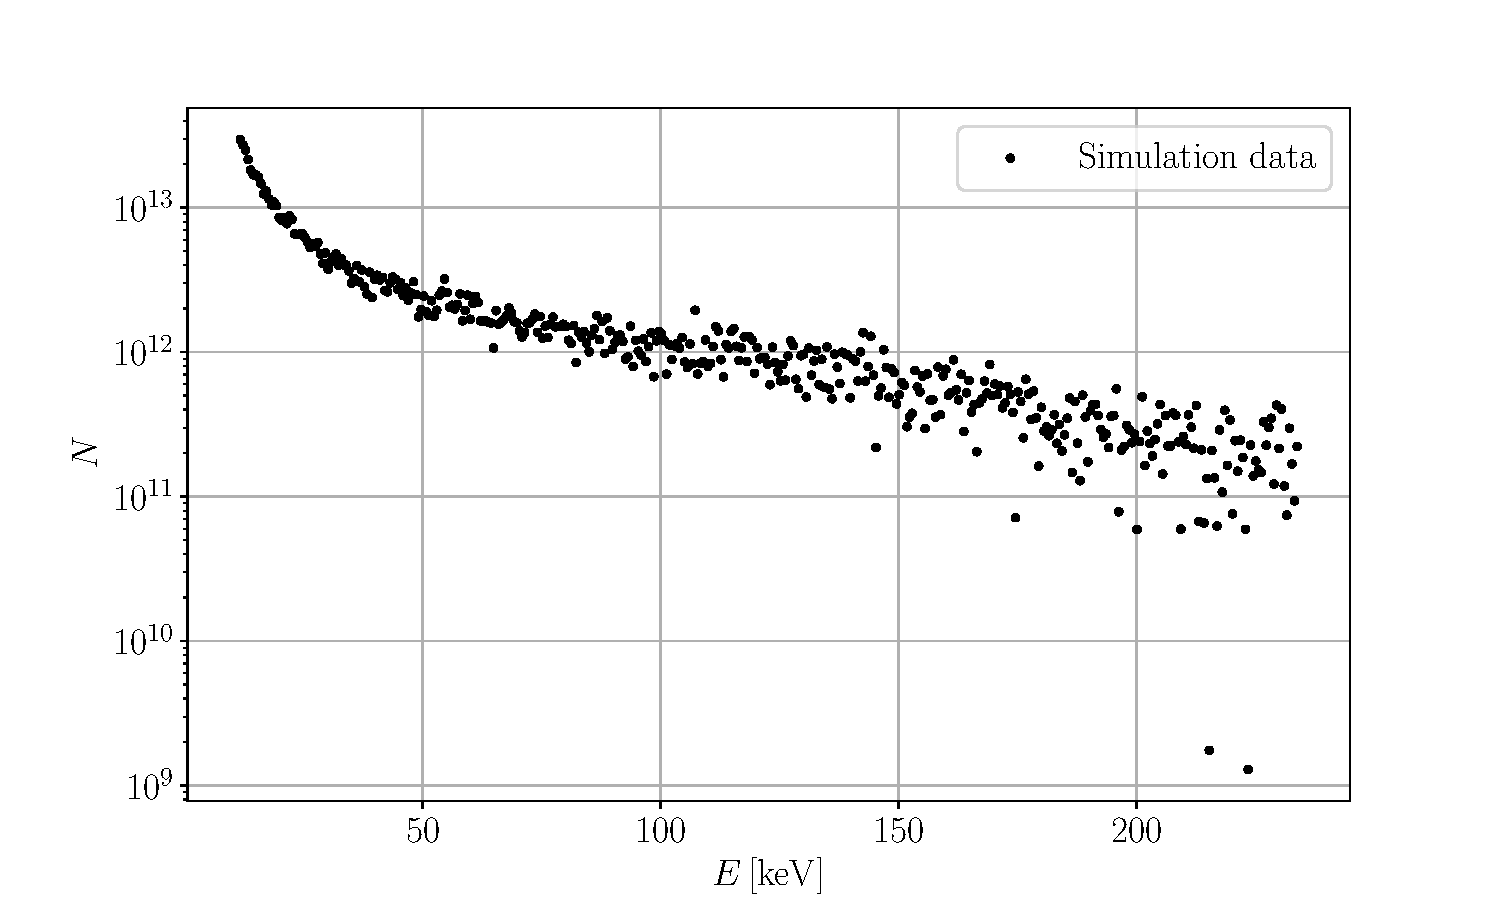
\includegraphics[width=0.9\textwidth]{figures/trimmed-hist}
	\caption{An example of trimmed histogram with simulation parameters $I=10^{19}\,\mathrm{W.cm}^{-2}$, $L=0.1\,\mathrm{\mu m}$ and $\alpha = 10$°.}
	\label{fig:trimmed-hist}
\end{figure}

The result of the cut-off of histogram \ref{fig:example-histogram} can be seen in figure \ref{fig:trimmed-hist}. Notice that the data show non-symmetrical noise in the part of the spectrum with the highest energies. This can be attributed to the logarithmic scale which can skew and seemingly magnify the noise for lower electron counts. 

For the purpose of the fitting, it is suitable to approximate the histogram data as points with $x$ values equal to the centre of the corresponding histogram bin and $y$ value equal to count.

The Jacquelin method was implemented in Python programming language as a class with number of exponential terms as a parameter. However, the lack of the numerical stability for more exponential terms usually causes issues for more than three terms because of reasons discussed at the end of chapter \ref{ch:temp-fitting-theory}.

As we said multiple times before, apart from the hot electron distribution, the other present distributions are not important to us. It is reasonable to assume, that the quality of fit is improved, if the fitted part is as small as possible but still containing the section where hot electrons dominate.

That being said, the next step aims to cut (or rather ignore) the beginning histogram once again, but now in a more sophisticated way. We found out that the majority of the histograms can be fit by the three-exponential Jacquelin method. Even though some do not have three distributions present, the fit usually does not fail and gives us valuable information.


We start by fitting the histogram using the three-exponential Jacquelin method. Of the three, there is one exponential distribution dominant for small energies. The corresponding electron distribution temperature is the lowest of all three distributions. We can quantify the energy $E_{\mathrm{crit}}$ at which the two most dominant terms are equal using equation:
\begin{equation}
	E_{\mathrm{crit}} = \frac{\ln{\left(a_1/a_2\right)}}{b_2-b_1}
\end{equation}
and use it as threshold for the cut-off. 

The basic illustration of the idea we just described can be seen in figure \ref{fig:3exp-fit-cut-example}. Note that $E_{\mathrm{crit}}$ intersects the fitted curve approximately in the middle of the arc where one exponential term is equal to the other. To make the lowest temperature electron distribution insignificant, the cut-off is made even a little further right. The hot electron temperature $T_\mathrm{hot}$ calculated by:
\begin{equation}
	T_{\mathrm{hot}} = -\frac{1}{b_3},
\end{equation}
where $b_3$ is the highest negative exponential coefficient of the whole fit. The attribute \textit{negative} is emphasized for practical reasons, because it is not guaranteed. The other cases have to be handled separately. The standard error $\Delta T_\mathrm{hot}$ can then be calculated as:
\begin{equation}
	\Delta T_\mathrm{hot} = \frac{\Delta b_3}{b_3^2} = T_\mathrm{hot}^2\Delta b_3,
\end{equation}
where $\Delta b_3$ is the standard error of $b_3$. 
	
\begin{figure}[ht]
	\centering
	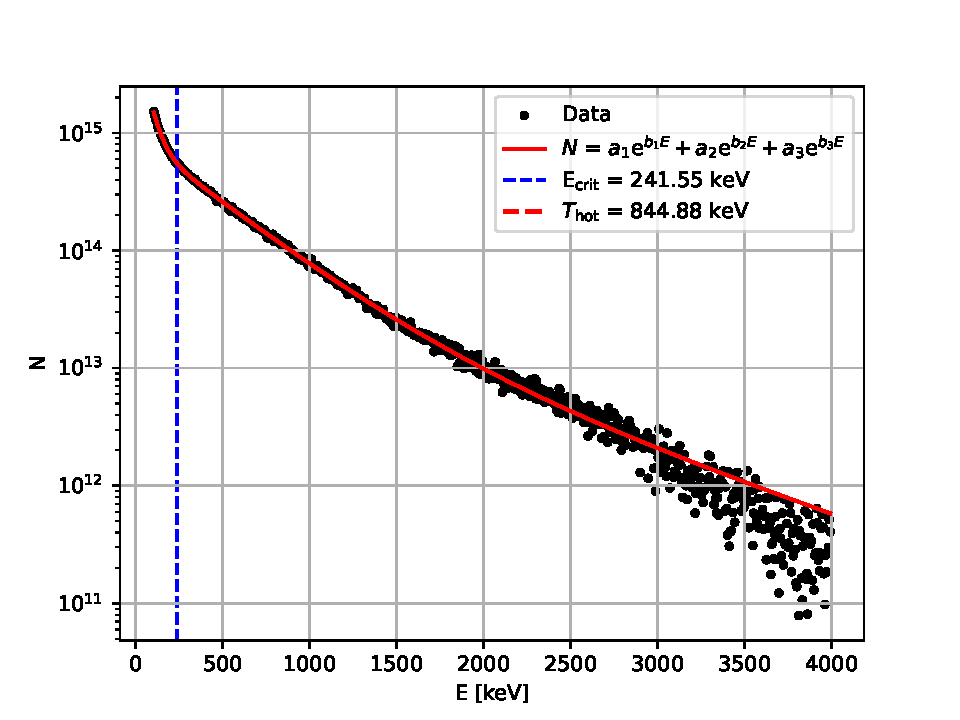
\includegraphics[width=0.9\textwidth]{figures/hist_1e19_060_30_3exp}
	\caption{An example of histogram with simulation parameters $I=10^{19}\,\mathrm{W.cm}^{-2}$, $L=0.6\,\mathrm{\mu m}$ and $\alpha = 30$° fitted with three-exponential Jacquelin method. The energy $E_{\mathrm{crit}}$ is highlighted.}
	\label{fig:3exp-fit-cut-example}
\end{figure}

We found, that in most cases, it is now possible to perform the two-exponential Jacquelin method. The cut-off reduced the cumulative error of the partial sums, but what is more important, it justifies the lower number of the exponential terms. From our experience, the two-exponential Jacquelin fit is generally also a little bit more stable. 

The "removal" of the lowest temperature electron distribution we just defined is analogical to the one described earlier in chapter \ref{ch:temp-fitting-theory} in section about fitting multi-exponential functions. Here we do a similar step but from the opposite end.

The two exponential fit performed on the cut version of the histogram in figure \ref{fig:3exp-fit-cut-example} with the cut-off part plotted but not fitted is shown in figure \ref{fig:2exp-fit-example}. It is possible to see that $T_{\mathrm{hot}}$ estimate is lower than it was before. Whether two-exponential Jacquelin method on cut histogram provides better $T_{\mathrm{hot}}$ estimates compared to three-exponential Jacquelin method on the original histogram will be a part of a later discussion.

As a last step of our strategy, we now use an iterative algorithm to converge to the best solution from the initial guess provided by the last fit. It can be argued that this step is not truly necessary, because we do not have a good reason to assume that the ill-conditioning of this problem disappeared by few cuts. Nevertheless, it will provide an additional insight to the later discussion and comparison of intermediate estimates of $T_{\mathrm{hot}}$.
\begin{figure}[t]
	\centering
	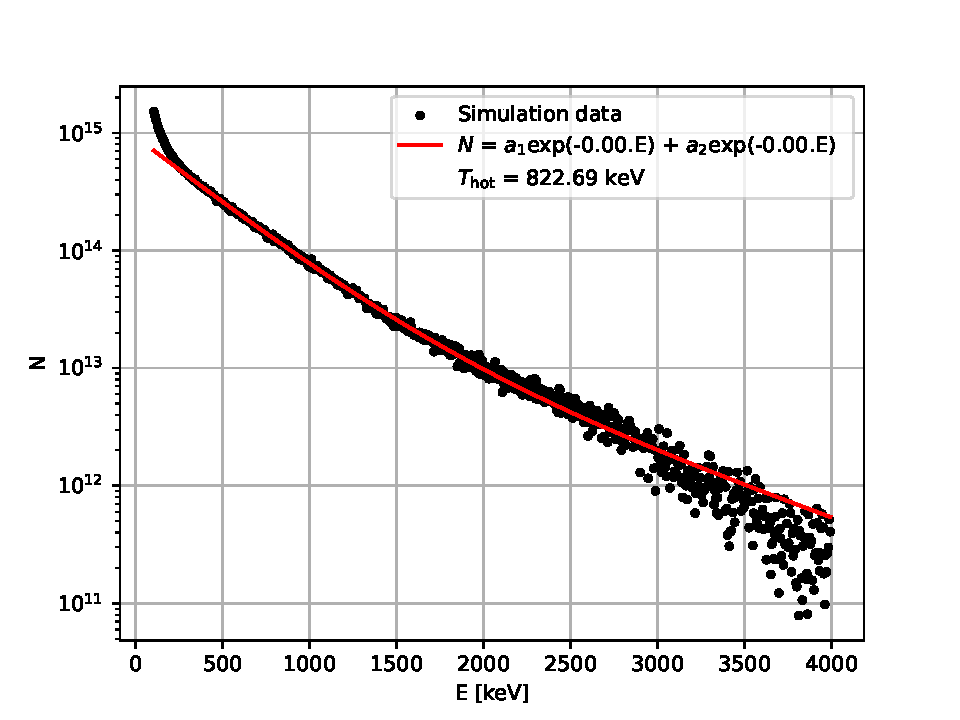
\includegraphics[width=0.9\textwidth]{figures/hist_1e19_060_30_2exp}
	\caption{An example of histogram with simulation parameters $I=10^{19}\,\mathrm{W.cm}^{-2}$, $L=0.6\,\mathrm{\mu m}$ and $\alpha = 30$° fitted with three-exponential Jacquelin method.}
	\label{fig:2exp-fit-example}
\end{figure}



